\documentclass[letterpaper,12pt,fleqn]{article}
\usepackage{matharticle}
\usepackage{tikz}
\usepackage{pgfplots}
\pgfplotsset{compat=1.16}
\renewcommand{\a}{\alpha}
\renewcommand{\l}{\lambda}
\newcommand{\p}{\phi}
\newcommand{\T}{\mathscr{T}}
\renewcommand{\i}{\iota}
\pagestyle{plain}
\begin{document}
\section*{Fundamental Groups of Topological Spaces}

Every topological space has a fundamental group.  Homeomorphic spaces have isomorphic fundamental groups.  This
allows for an extra technique for determining that two spaces are not homeomorphic when all of the other
topological properties seem to be preserved by continuous functions.  For example:
\begin{enumerate}
\item \(\R^2\) and \(\R^3\)
\item \(S^2\), \(T\), and \(T\#T\)
\end{enumerate}

\begin{definition}[Group]
  A \emph{group} \((G,*)\) is a set \(G\) with binary operator \(*\) such that the following axioms are satisfied:
  \begin{enumerate}
  \item Associative: \((a*b)*c=a*(b*c)\)
  \item Identity: \(a*e=e*a\)
  \item Inverse: \(a*a'=a'*a=e\)
  \end{enumerate}
\end{definition}

\begin{definition}[Abelian Group]
  An \emph{abelian} group \((G,*)\) is a group whose binary operator is commutative:
  \[a*b=b*a\]
\end{definition}

\begin{definition}[Homomorphic]
  To say that two groups \((G,*)\) and \((G',*')\) are \emph{homomorphic} means that there exists a function
  \(\p:G\to G'\) such that:
  \[\p(x*y)=\p(x)*'\p(y)\]
  Such a \(\p\) is called a \emph{homomorphism}.
\end{definition}

\begin{properties}[Homomorphism]
  Let \(f:G\to G'\) be a homomorphism:
  \begin{enumerate}
  \item The \emph{kernel} of \(f\) is the preimage of the identity of \(G'\): \(f^{-1}(e')\), and it is a subgroup
    of \(G\).
  \item The image of \(f\): \(f(G)\), is a subgroup of \(G'\).
  \item If \(f\) is injective (kernel=\(\set{e}\)) then it is called a \emph{monomorphism}.
  \item If \(f\) is surjective then it is called an \emph{epimorphism}.
  \item If \(f\) is bijective then it is called an \emph{isomorphism}.
  \end{enumerate}
\end{properties}

\begin{definition}[Isomorphism]
  To say that two groups \((G,*)\) and \((G',*')\) are \emph{isomorphic} means that there exists an isomorphism
  \(\p:G\to G'\).
\end{definition}

\begin{definition}[Coset]
  Let \(H\) be a subgroup of a group \(G\).  The \emph{left cosets} of \(H\) in \(G\) are defined as:
  \[xH=\setb{xh}{h\in H}\]
  for all \(x\in X\).  The left cosets of \(H\) form a partition of \(G\).  Similarly, the \emph{right cosets}
  \(Hx\) also form a partition of \(G\).
\end{definition}

\begin{definition}[Normal]
  To say that a subgroup \(H\) of a group \(G\) is \emph{normal} in \(G\) means for all \(x\in G\) and all
  \(h\in H\), \(xhx^{-1}\in H\).  In this case, for all \(x\in G\), \(xH=Hx\).
\end{definition}

\begin{definition}[Quotient]
  Let \(H\) be a normal subgroup of a group \(G\) and define the binary operator:
  \[(xH)(yH)=(xy)H\]
  The partition of \(G\) by \(H\) with this operation forms a group denoted by \(G/H\) and called the
  \emph{quotient group} of \(G\) by \(H\).
\end{definition}

\begin{properties}[Quotient]
  Let \(G/H\) be the quotient group of \(G\) by \(H\):
  \begin{enumerate}
  \item The function \(f:G\to G/H\) defined by \(f(x)=xH\) is an epimorphism with kernel \(H\).
  \end{enumerate}
\end{properties}

\begin{notation}
  \(I=[0,1]\subset\R\) imbued with the subspace topology.
\end{notation}

\begin{definition}[Homotopy]
  Let \(X\) and \(Y\) be topological spaces and let \(f_1,f_2:X\to Y\) be continuous.  To say that \(f_1\) and
  \(f_2\) are \emph{homotopic}, denoted by \(f_1\simeq f_2\), means that there exists a continuous function
  \(F:X\times I\to Y\) such that \(F(x,0)=f_1(x)\) and \(F(x,1)=f_2(x)\).  Such a function \(F\) is called a
  \emph{homotopy} between \(f_1\) and \(f_2\).
\end{definition}

\begin{definition}[Nulhomotopic]
  Let \(X\) and \(Y\) be topological spaces and let \(f_1:X\to Y\) be continuous.  To say that \(f_1\) is
  \emph{nulhomotopic} means that there exists a constant function \(f_2:X\to Y\) such that \(f_1\simeq f_2\).
\end{definition}

A homotopy can be viewed as a continuous deformation of \(f_1\) into \(f_2\) via a parameterized family of
continuous functions.

\begin{example}[Vertical Shift]
  Let \(X=Y=I\) and let \(f_1(x)=0\) and \(f_2(x)=1\).  Consider \(F:I\times I\to I\) defined by
  \(F(x,k)=\pi_{I}(x,k)=k\).  Note that the projection map is known to be continuous:

  \begin{tikzpicture}
    \begin{axis}[
        xmin=0,
        xmax=1,
        ymin=0,
        ymax=1,
        axis lines*=middle,
        xtick={0,1},
        ytick={0,1},
        ytick={0,1/5,2/5,3/5,4/5,1},
        yticklabels={\(0\),\(\frac{1}{5}\),\(\frac{2}{5}\),\(\frac{3}{5}\),\(\frac{4}{5}\),\(1\)},
        xlabel={\(I\)},
        ylabel={\(I\)},
        ylabel style={rotate=-90},
        legend pos=outer north east,
        legend cell align=left,
        clip=false
      ]
      \addplot [domain=0:1,red] {0};
      \addplot [domain=0:1,green] {1};
      \addplot [domain=0:1,dashed] {0.2};
      \addplot [domain=0:1,dashed] {0.4};
      \addplot [domain=0:1,dashed] {0.6};
      \addplot [domain=0:1,dashed] {0.8};
      \legend{\(f_1(x)=0\),\(f_2(x)=1\)};
    \end{axis}
  \end{tikzpicture}
\end{example}

\begin{lemma}
  Let \(X\) and \(Y\) be topological spaces and let \(f:X\to Y\) be continuous.  For all \(A\subset X\),
  \(\restrict{f}{A}\) is continuous.
\end{lemma}

\begin{proof}
  Assume \(A\subset X\) and assume \(V\) is open in \(Y\).  Since \(f\) is continuous, \(f^{-1}(V)\) is open in
  \(X\).  Furthermore, by definition of the subspace topology, \(\restrict{f}{A}^{-1}(V)=f^{-1}(V)\cap A\) is open
  in \(A\).  Therefore \(\restrict{f}{A}\) is continuous.
\end{proof}

\begin{corollary}
  Let \(X\) and \(Y\) be topological spaces, let \(f_1,f_2:X\to Y\) be continuous, and let \(F:X\times I\to Y\) be
  a homotopy between \(f_1\) and \(f_2\).  For all \(k\in I\), define \(f_k(x)=F(x,k)=\restrict{F}{X\times\set{k}}\).
  All of the \(f_k\) are continuous.
\end{corollary}

\begin{proof}
  Since \(F\) is a homotopy, it is continuous.  Therefore \(\restrict{F}{X\times\set{k}}=F(x,k)=f_k(x)\) is
  continuous.
\end{proof}

\begin{example}[Horizontal Shift]
  Let \(X=I\) and and \(Y=\R\), and let \(f_1(x)=\sin(2\pi x)\) and \(f_2(x)=\cos(2\pi x)\).  Consider \(F:I\times
  I\to\R\) defined by \(F(x,k)=\sin\left(2\pi x+k\frac{\pi}{2}\right)\).

  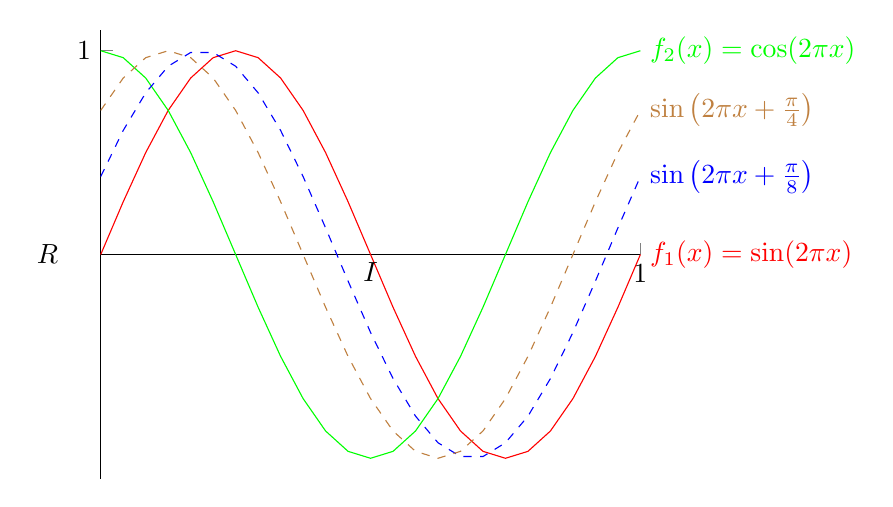
\begin{tikzpicture}
    \begin{axis}[
        xmin=0,
        xmax=1,
        ymin=-1.1,
        ymax=1.1,
        axis lines*=middle,
        xtick={0,1},
        ytick={0,1},
        xlabel={\(I\)},
        ylabel={\(R\)},
        xlabel style={above=0cm},
        ylabel style={rotate=-90},
        clip=false
      ]
      \addplot [domain=0:1,red] {sin(deg(2*pi*x))} node [right] {\(f_1(x)=\sin(2\pi x)\)};
      \addplot [domain=0:1,green] {cos(deg(2*pi*x))} node [right] {\(f_2(x)=\cos(2\pi x)\)};
      \addplot [domain=0:1,blue,dashed] {sin(deg(2*pi*x+pi/8))}
      node [right] {\(\sin\left(2\pi x+\frac{\pi}{8}\right)\)};
      \addplot [domain=0:1,brown,dashed] {sin(deg(2*pi*x+pi/4))}
      node [right] {\(\sin\left(2\pi x+\frac{\pi}{4}\right)\)};
    \end{axis}
  \end{tikzpicture}
\end{example}

\begin{example}[Scaling]
  Let \(X=I\) and and \(Y=\R\), and let \(f_1(x)=\sin(2\pi x)+1\) and \(f_2(x)=0\).  Consider \(F:I\times
  I\to\R\) defined by \(F(x,k)=(1-k)[\sin(2\pi x)+1]\).

  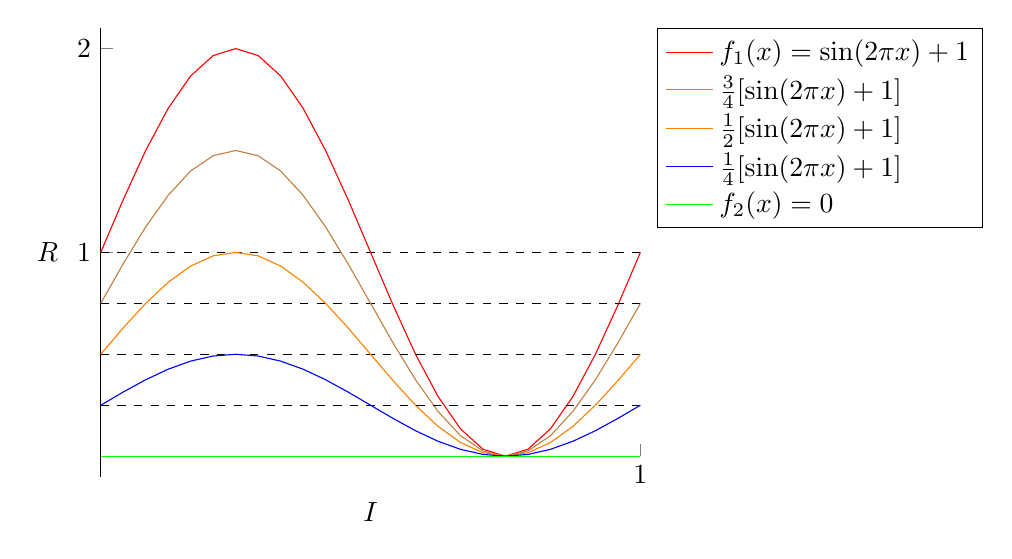
\begin{tikzpicture}
    \begin{axis}[
        xmin=0,
        xmax=1,
        ymin=-0.1,
        ymax=2.1,
        axis lines*=middle,
        xtick={0,1,2},
        ytick={0,1,2},
        xlabel={\(I\)},
        ylabel={\(R\)},
        ylabel style={rotate=-90},
        legend pos=outer north east,
        legend cell align=left,
        clip=false
      ]
      \draw [dashed] (0,1) -- (1,1);
      \addplot [domain=0:1,red] {sin(deg(2*pi*x))+1};
      \draw [dashed] (0,3/4) -- (1,3/4);
      \addplot [domain=0:1,brown] {(3/4)*(sin(deg(2*pi*x))+1)};
      \draw [dashed] (0,1/2) -- (1,1/2);
      \addplot [domain=0:1,orange] {(1/2)*(sin(deg(2*pi*x))+1)};
      \draw [dashed] (0,1/4) -- (1,1/4);
      \addplot [domain=0:1,blue] {(1/4)*(sin(deg(2*pi*x))+1)};
      \addplot [domain=0:1,green] {0};
      \legend{\(f_1(x)=\sin(2\pi x)+1\),\(\frac{3}{4}[\sin(2\pi x)+1]\),\(\frac{1}{2}[\sin(2\pi x)+1]\),
        \(\frac{1}{4}[\sin(2\pi x)+1]\),\(f_2(x)=0\)}
    \end{axis}
  \end{tikzpicture}
\end{example}

Based on the past examples it is tempting to make the theorem and equivalence.  But, a function of a product
space is not necessarily continuous if it is continuous in each variable separately.

\begin{example}
  Let \(F:\R\times\R\to\R\) be defined by:
  \[F(x,y)=\begin{cases}
  \frac{xy}{x^2+y^2}, & (x,y)\ne(0,0) \\
  0, & (x,y)=(0,0)
  \end{cases}\]
  Note that \(F\) is continuous in both \(x\) and \(y\) separately, but is discontinuous at \((0,0)\) along the
  line \(y=x\):
  \[F(x,x)=\begin{cases}
  \frac{1}{2}, & (x,y)\ne(0,0) \\
  0, & (x,y)=(0,0)
  \end{cases}\]
\end{example}

\begin{lemma}
  Let \(X\) and \(Y\) be topological spaces and let \(h:X\times Y\to X\times Y\) be defined by
  \(h(x,y)=(f(x),g(y))\) where \(f:X\to X\) and \(g:Y\to Y\) are continuous.  Then \(h\) is continuous.
\end{lemma}

\begin{proof}
  Assume that \(W\in\T_{X\times Y}\).  This means that \(W=\bigcup_{\a\in\l}(U_{\a}\times V_{\a})\) where
  the \(U_{\a}\in\T_X\) and the \(V_{\a}\in\T_Y\).  Now:
  \begin{align*}
    h^{-1}(W) &= h^{-1}\left[\bigcup_{\a\in\l}(U_{\a}\times V_{\a})\right] \\
    &= \bigcup_{\a\in\l}h^{-1}(U_{\a}\times V_{\a}) \\
    &= \bigcup_{\a\in\l}[f^{-1}(U_{\a})\times g^{-1}(V_{\a})] \\
    & \in\T_{X\times Y}
  \end{align*}
  Therefore \(h\) is continuous.
\end{proof}

\begin{corollary}
  Let \(X\), \(Y\), and \(\Z\) be topological spaces and let \(F:X\times Y\to Z\), \(f:X\to X\), and \(g:Y\to Y\)
  be continuous.  The function \(G:X\times Y\to Z\) defined by \(G(x,y)=F(f(x),g(y))\) is continuous.
\end{corollary}

\begin{proof}
  Let \(h:X\times Y\to X\times Y\) be defined by \(h(x,y)=(f(x),g(y))\).  This means that \(h\) is continuous.
  Therefore \(G=F\circ h\) is continuous.
\end{proof}

\begin{corollary}
  Let \(X\) and \(Y\) be topological spaces and let \(f_1,f_2:X\to Y\) be homotopic.  If \(g:Y\to Z\) is
  continuous then \(g\circ f_1\) is homotopic to \(g\circ f_2\) in \(Z\).  In particular, if \(F\) is a homotopy
  between \(f_1\) and \(f_2\) then \(g\circ F\) is a homotopy between \(g\circ f_1\) and \(g\circ f_2\).
\end{corollary}

\begin{proof}
  Assume that \(F\) is a homotopy between \(f_1\) and \(f_2\) in \(Y\).  This means that \(F:X\times I\to Y\) is
  continuous and \(F(x,0)=f_1(x)\) and \(F(x,1)=f_2(x)\).  So, since \(F\) and \(g\) are continuous,
  \(g\circ F\) is continuous in \(Z\).  Furthermore, \((g\circ F)(x,0)=g(F(x,0))=g(f_1(x))=(g\circ f_1)(x)\) and
  \((g\circ F)(x,1)=g(F(x,1))=g(f_2(x))=(g\circ f_2)(x)\).  Therefore \(g\circ F\) is a homotopy between \(g\circ f_1\)
  and \(g\circ f_2\).
\end{proof}

\begin{theorem}
  Homotopic is an equivalence relation.
\end{theorem}

\begin{proof}
  Let \(X\) and \(Y\) be topological spaces and let \(f_1,f_2,f_3:X\to Y\) be continuous:
  \begin{description}
  \item[Reflexive:] Consider the function \(F:X\times I\to Y\) defined by \(F(x,k)=f_1(x)\).

    Assume that \(V\in\T_Y\).  Since \(f\) is continuous, \(f_1^{-1}(V)\in\T_X\).  Furthermore,
    \(F^{-1}(V)=f_1^{-1}(V)\times I\in\T_{X\times I}\).  Thus \(F\) is continuous, \(F(x,0)=f_1(x)\), and
    \(F(x,1)=f_1\), and hence \(F\) is a homotopy between \(f_1\) and \(f_1\).  Therefore \(f_1\simeq f_1\).

  \item[Symmetric:]  Assume that \(f_1\simeq f_2\).

    This means that there exists a continuous function \(F:X\times I\to Y\) between \(f_1\) and \(f_2\) such that
    \(F(x,0)=f_1(x)\) and \(F(x,1)=f_2(x)\).  Let \(G:X\times I\to Y\) be defined by \(G(x,k)=F(x,1-k)\).  Thus,
    \(G\) is continuous.  Furthermore, \(G(x,0)=F(x,1)=f_2(x)\) and \(G(x,1)=F(x,0)=f_1(x)\).  Therefore \(G\) is a
    homotopy between \(f_2\) and \(f_1\) and thus \(f_2\simeq f_1\).

  \item[Transitive:]  Assume that \(f_1\simeq f_2\) and \(f_2\simeq f_3\).

    Assume that \(F\) is a homotopy between \(f_1\) and \(f_2\) and \(G\) is a homotopy between \(f_2\) and \(f_3\)
    and defined the function \(G:X\times I\to Y\) as:
    \[H(x,k)=\begin{cases}
    F(x,2k), & k\in\left[0,\frac{1}{2}\right] \\
    G(x,2k-1), & k\in\left[\frac{1}{2},1\right] \\
    \end{cases}\]
    Note that \(F\) and \(G\) agree for \(k=\frac{1}{2}\), so by the pasting lemma, \(H\) is continuous.
    Furthermore, \(H(x,0)=F(x,0)=f_1(x)\) and \(H(x,1)=G(x,1)=f_3(x)\).  Therefore \(H\) is a homotopy between
    \(f_1\) and \(f_3\) and thus \(f_1\simeq f_3\).
  \end{description}
\end{proof}

\begin{notation}
  Let \(X\) and \(Y\) be a topological spaces and let \(f:X\to Y\) be continuous.  The equivalence class containing
  all continuous functions that are homotopic to \(f\) is denoted by \([f]\):
  \[[f]=\setb{g:X\to Y}{g\ \text{is continuous and}\ g\simeq f}\]
\end{notation}

In particular, any two continuous functions \(f,g:X\to\R^2\) are homotopic via the so-called \emph{straight-line}
homotopy:
\[F(x,k)=(1-k)f(x)+kg(x)\]
It is called this because each \(f(x)\) moves to its corresponding \(g(x)\) along a straight line.

This can be generalized.

\begin{definition}[Convex]
  Let \(A\) be a subspace of \(R^n\).  To say that \(A\) is convex means that for any two points \(a,b\in A\) and
  the function \(f:\R^n\to\R^n\) defined as \(f(t)=(1-t)a+tb\), \(f(A)\subset A\).
\end{definition}

Thus, if \(A\subset\R^n\) is convex then any two continuous functions in \(A\) are homotopic via the straight-line
homotopy.

\begin{definition}[Path]
  Let \(X\) be a topological space and let \(x_0,x_1\in X\).  To say that a continuous map \(f:I\to X\) is a
  \emph{path} from \(x_0\) (the \emph{initial} point) to \(x_1\) (the \emph{final} point) means that \(f(0)=x_0\)
  and \(f(1)=x_1\).
\end{definition}

\begin{example}[Paths]
  Let \(X=\R^2\) and let \(x_0=(0,0)\) and \(x_1=(1,-1)\):

  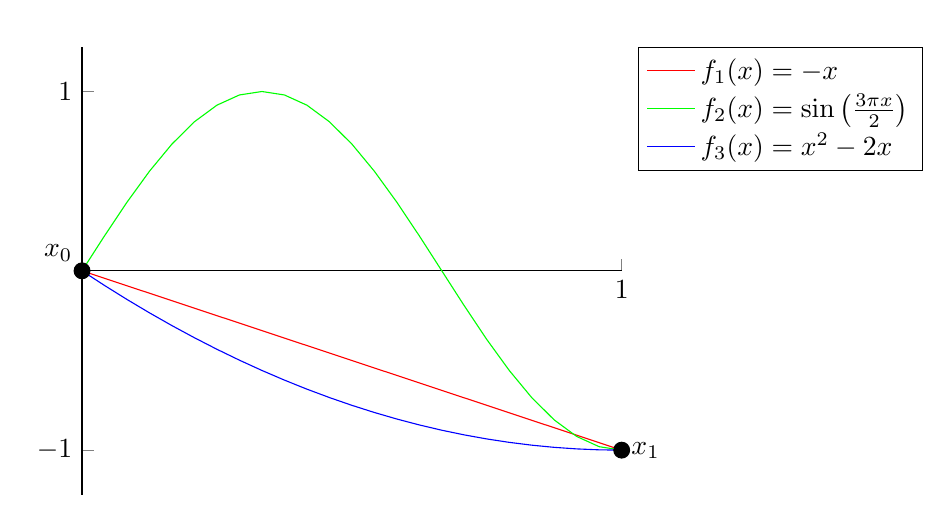
\begin{tikzpicture}
    \begin{axis}[
        xmin=0,
        xmax=1,
        ymin=-2.5,
        ymax=2.5,
        axis lines*=middle,
        xtick={0,1},
        ytick={-2,0,2},
        yticklabels={\(-1\),\(0\),\(1\)},
        legend pos=outer north east,
        legend cell align=left,
        clip=false
      ]
      \addplot [domain=0:1,red] {-2*x};
      \addplot [domain=0:1,green] {2*sin(deg((3*pi/2)*x))};
      \addplot [domain=0:1,blue] {2*((x-1)^2-1)};
      \node [draw,circle,fill,inner sep=0,minimum size=0.2cm] at (0,0) {};
      \node [above left] at (0,0) {\(x_0\)};
      \node [draw,circle,fill,inner sep=0,minimum size=0.2cm] at (1,-2) {};
      \node [right] at (1,-2) {\(x_1\)};
      \legend{\(f_1(x)=-x\),\(f_2(x)=\sin\left(\frac{3\pi x}{2}\right)\),\(f_3(x)=x^2-2x\)};
      \node (R1) at (1,0) {};
      \node (R2) at (0,2.5) {};
    \end{axis}
    \node [right] at (R1) {\(\R\)};
    \node [above] at (R2) {\(\R\)};
  \end{tikzpicture}
\end{example}

\begin{definition}[Path Homotopy]
  Let \(X\) be a topological space and let \(f_1\) and \(f_2\) be two paths in \(X\).  To say that \(f_1\) and
  \(f_2\) are \emph{path homotopic} means that they have the same initial point \(x_0\) and the same final point
  \(x_1\) and there exists a continuous map \(F:I\times I\to X\) such that:
  \begin{enumerate}
  \item \(F(s,0)=f_1(s)\) and \(F(s,1)=f_2(s)\)
  \item \(F(0,t)=x_0\) and \(F(1,t)=x_1\)
  \end{enumerate}
\end{definition}

\begin{example}[Path Homotopy]
  Let \(X=\R^2\) and let \(x_0=(0,0)\) and \(x_1=(1,1)\):

  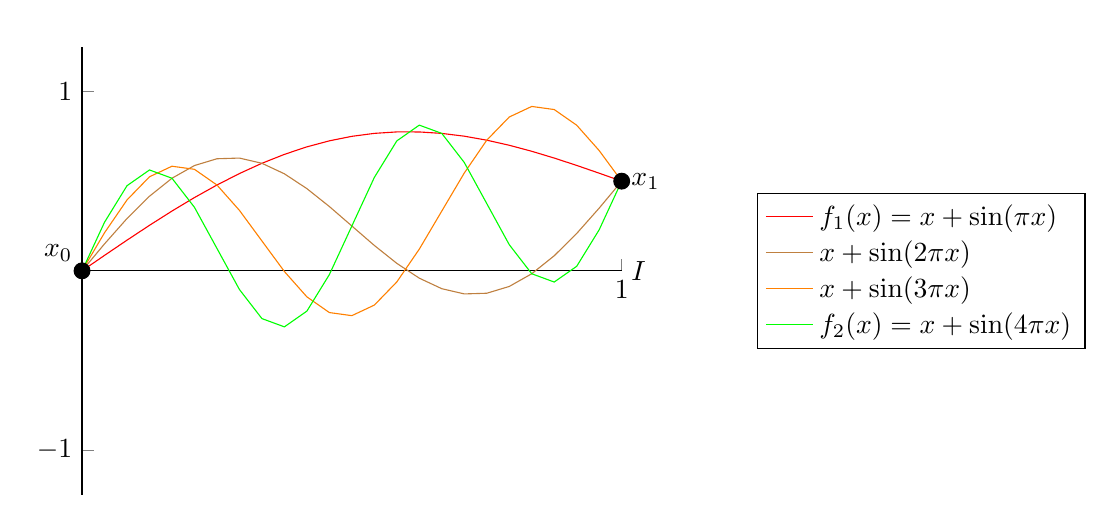
\begin{tikzpicture}
    \begin{axis}[
        xmin=0,
        xmax=1,
        ymin=-2.5,
        ymax=2.5,
        axis lines*=middle,
        xtick={0,1},
        ytick={-2,0,2},
        yticklabels={\(-1\),\(0\),\(1\)},
        legend style={at={(1.25,0.5)},anchor=west},
        legend cell align=left,
        clip=false
      ]
      \addplot [domain=0:1,red] {x+sin(deg(pi*x))};
      \addplot [domain=0:1,brown] {x+sin(deg(2*pi*x))};
      \addplot [domain=0:1,orange] {x+sin(deg(3*pi*x))};
      \addplot [domain=0:1,green] {x+sin(deg(4*pi*x))};
      \node [draw,circle,fill,inner sep=0,minimum size=0.2cm] at (0,0) {};
      \node [above left] at (0,0) {\(x_0\)};
      \node [draw,circle,fill,inner sep=0,minimum size=0.2cm] at (1,1) {};
      \node [right] at (1,1) {\(x_1\)};
      \legend{\(f_1(x)=x+\sin(\pi x)\),\(x+\sin(2\pi x)\),\(x+\sin(3\pi x)\),\(f_2(x)=x+\sin(4\pi x)\)}
      \node (I) at (1,0) {};
      \node (R) at (0,2.5) {};
    \end{axis}
    \node [right] at (I) {\(I\)};
    \node [above] at (R) {\(\R\)};
  \end{tikzpicture}
\end{example}

Note that path homotopic is also an equivalence relation.

\begin{definition}
  Let \(X\) be a topological space and let \(f_1\) be a path in \(X\) from \(x_0\) to \(x_1\) and let \(f_2\) be a
  path in \(X\) from \(x_1\) to \(x_2\).  The \emph{product} of \(f_1\) and \(f_2\) is given by:
  \[f_1*f_2=\begin{cases}
  f_1(2k), & k\in\left[0,\frac{1}{2}\right] \\
  f_2(2k-1), & k\in\left[\frac{1}{2},1\right] \\
  \end{cases}\]
\end{definition}

Note that \(f_1\) and \(f_2\) agree at \(k=\frac{1}{2}\)
\((f_1\left(\frac{1}{2}\right)=f_2\left(\frac{1}{2}\right)=x_1)\), so by the pasting lemma, \(f_1*f_2\) is
continuous and thus a path in \(X\) from \(x_0\) to \(x_2\).

The product operator is not a binary operator because it is only defined on paths where \(f_1(1)=f_2(0)\).  Thus,
the product operator creates a \emph{groupoid}.

\begin{lemma}
  Let \(X\) and \(Y\) be topological spaces and let \(f_1\) and \(f_2\) be two paths in \(X\) such that
  \(f_1(1)=f_2(0)\), and let \(g:X\to Y\) be continuous:
  \[g\circ(f_1*f_2)=(g\circ f_1)*(g\circ f_2)\]
\end{lemma}

\begin{proof}
  Let \(f_1\) is a path from \(x_0\) to \(x_1\) and let \(f_2\) be a path from \(x_1\) to \(x_2\).
  \begin{description}
  \item[case 1:] \(k\in\left[0,\frac{1}{2}\right]\)
    \[(g\circ(f_1*f_2))(k)=g((f_1*f_2)(k))=g(f_1(k))=(g\circ f_1)(k)=((g\circ f_1)*(g\circ f_2))(k)\]
  \item[case 2:] \(k\in\left[\frac{1}{2},1\right]\)
    \[(g\circ(f_1*f_2))(k)=g((f_1*f_2)(k))=g(f_2(k))=(g\circ f_2)(k)=((g\circ f_1)*(g\circ f_2))(k)\]
  \end{description}

  At \(k=\frac{1}{2}\):
  \begin{gather*}
    (g\circ f_1)\left(\frac{1}{2}\right)=g(f_1(1))=x_1 \\
    \\
    (g\circ f_2)\left(\frac{1}{2}\right)=g(f_2(0))=x_1
  \end{gather*}
  So the function agree on the intersection.  Furthermore:
  \begin{gather*}
    ((g\circ f_1)*(g\circ f_2))(0) = g(f_1(0))=x_0 \\
    \\
    ((g\circ f_1)*(g\circ f_2))(1) = g(f_2(1))=x_2 \\
  \end{gather*}
  And so the initial and final points are correct.
\end{proof}

\begin{notation}
  Let \(X\) be a topological space and let \(x\in X\).  The constant path that maps all of \(I\) to \(x\) is
  denoted by \(e_x\).
\end{notation}

\begin{lemma}
  Let \(X\) be topological space and let \(f\) be a path from \(x_0\) to \(x_1\) in \(X\):
  \begin{enumerate}
  \item \([f]\circ e_0=[e_{x_0}]\)
  \item \([f]\circ e_1=[e_{x_1}]\)
  \end{enumerate}
\end{lemma}

\begin{proof}
  Assume that \(f\) is a path from \(x_0\) to \(x_1\) in \(X\):
  \begin{enumerate}
    \item \((f\circ e_0)(j)=f(e_0(j))=f(0)=x_0\)
    \item \((f\circ e_1)(j)=f(e_1(j))=f(1)=x_1\)
  \end{enumerate}
\end{proof}

\begin{definition}[Reverse]
  Let \(X\) be a topological space and let \(f\) be a path from \(x_0\) to \(x_1\) in \(X\).  The \emph{reverse} of
  \(f\) is the path from \(x_1\) to \(x_0\) in \(X\), denoted by \(\bar{f}\), is given by:
  \[\bar{f}(k)=f(1-k)\]
\end{definition}

\begin{lemma}
  Let \(X\) be a topological space.  For all paths \(f\) in \(X\):
  \begin{enumerate}
  \item \([f]\circ\i_I=[f]\)
  \item \([f]\circ\bar{\i}_I=[\bar{f}]\)
  \end{enumerate}
\end{lemma}

\begin{proof}
  Assume that \(f\) is a path in \(X\).
  \begin{enumerate}
  \item \((f\circ\i_I)(k)=f(\i_I(k))=f(k)\)
  \item \((f\circ\bar{\i_I})(k)=f(\bar{\i_I}(k))=f(1-k)=\bar{f}(k)\)
  \end{enumerate}
\end{proof}

\begin{theorem}
  Let \(X\) be a topological space and assume that \(f\), \(g\). and \(h\) be paths in \(X\) where \(f\) is a path
  from \(x_0\) to \(x_1\).  The product operator on a topological space \(X\) has the following properties:
  \begin{enumerate}
  \item Associative: \(([f]*[g])*[h]\) is defined if and only if \([f]*([g]*[h])\) is defined and if defined then
    they are equal.
  \item Identity: \([e_{x_0}]*[f]=[f]\) and \([f]*[e_{x_1}]=[f]\).
  \item Inverse: \([f]*[\bar{f}]=[e_{x_0}]\) and \([\bar{f}]*[f]=[e_{x_1}]\).
  \end{enumerate}
\end{theorem}

\begin{proof}
  \begin{enumerate}
  \item[]
  \item Associative:

  \item Identity:

    Consider the path \(e_0*\i_I\) as a path in \(I\) from \(0\) to \(1\).  Since \(I\) is convex, there exists a
    path homotopy \(F\) in \(I\) between \(\i_I\) and \(e_0*\i_I\).  This means that \(f\circ F\) is also a path
    homotopy in \(X\) between the paths \(f\circ\i_I=f\) and \(f\circ(e_0*\i_I)=(f\circ
    e_0)*(f\circ\i_I)=e_{x_0}*f\).

    Therefore \([f]=[e_{x_0}]*[f]\)

    Similarly, consider the path \(\i_I*e_1\) as a path in \(I\) from \(0\) to \(1\).  Since \(I\) is convex, there
    exists a path homotopy \(F\) in \(I\) between \(\i_I\) and \(\i_I*e_1\).  This means that \(f\circ F\) is also
    a path homotopy in \(X\) between the paths \(f\circ\i_I=f\) and \(f\circ(\i_I*e_1)=(f\circ\i_I)*(f\circ
    e_1)=f*e_{x_1}\).

    Therefore \([f]=[f]*[e_{x_1}]\)

  \item Inverse:

    Consider the path \(\i_I*\bar{\i}_I\) as a path in \(I\) from \(0\) to \(0\).  Since \(I\) is convex, there
    exists a path homotopy \(F\) in \(I\) between \(e_0\) and \(\i_I*\bar{\i}_I\).  This means that \(f\circ F\) is
    also a path homotopy in \(X\) between the paths \(f\circ e_0=e_{x_0}\) and
    \(f\circ(\i_I*\bar{\i}_I)=(f\circ\i_I)*(f\circ\bar{\i_I})=f*\bar{f}\).

    Therefore \([f]*[\bar{f}]=[e_{x_0}]\).

    Similarly, consider the path \(\bar{\i_I}*\i\) as a path in \(I\) from \(1\) to \(1\).  Since \(I\) is convex,
    there exists a path homotopy \(F\) in \(I\) between \(e_1\) and \(\bar{\i}_I*\i_I\).  This means that \(f\circ F\)
    is also a path homotopy in \(X\) between the paths \(f\circ e_1=e_{x_1}\) and
    \(f\circ(\bar{\i}_I*\i_I)=(f\circ\bar{\i}_I)*(f\circ\i_I)=\bar{f}*f\).

    Therefore \([\bar{f}]*[f]=[e_{x_1}]\).
  \end{enumerate}
\end{proof}

\begin{definition}[Loop]
  Let \(X\) be a topological space and let \(x_0\in X\).  A path in \(X\) whose initial and final point are both
  \(x_0\) is called a \emph{loop} in \(X\) based at \(x_0\).
\end{definition}

\begin{definition}[Fundamental Group]
  Let \(X\) be a topological space and let \(x_0\in X\).  The set of path homotopy classes of loops based at
  \(x_0\) along with the \(*\) operator is called the \emph{fundamental group} of \(X\) relative to the
  \emph{base point} \(x_0\) and is denoted by \(\pi_1(X,x_0)\).
\end{definition}

Note that \([e_{x_0}]\) is the identity element in the the fundamental group relative to \(x_0\).

\begin{theorem}
  Let \(A\) be a subspace of a topological space \(X\) and let \(x_0\in A\).  If \(A\) is convex then
  \[\pi_1(A,x_0)=\set{e_{x_0}}\]
\end{theorem}

\begin{proof}
  Assume that \(A\) is convex and assume that \(f\) is a loop based at \(x_0\).  Since \(A\) is convex,
  \(f\simeq (e_{x_0}\) by the straight-line homotopy.  Therefore \(f\in[e_{x_0}]\) and hence the fundamental
  group is trivial.
\end{proof}

\begin{corollary}
  All open balls in \(\R^n\) have the trivial fundamental group.
\end{corollary}

\begin{definition}
  Let \(X\) be a topological space and let \(\a\) be a path in \(X\) between \(x_0\) and \(x_1\).  Define the
  function \(\hat{\a}:\pi_1(X,x_0)\to\pi_1(X,x_1)\) as follows:
  \[\hat{\a}([f])=[\bar{\a}]*[f]*[\a]\]
\end{definition}

\begin{theorem}
  Let \(X\) be a topological space and let \(\a\) be a path in \(X\) between \(x_0\) and \(x_1\).  \(\hat(\a)\)
  is a group isomorphism.
\end{theorem}

\begin{proof}
  Assume that \(f,g\in\pi_1(X,x_0)\):
  \begin{align*}
    \hat{\a}([f])*\hat{\a}(g) &= ([\bar{\a}]*[f]*[\a])*([\bar{\a}]*[g]*[\a]) \\
    &= [\bar{\a}]*[f]*[e_{x_1}]*[g]*[\a] \\
    &= [\bar{\a}]*[f]*[g]*[\a] \\
    &= \hat{\a}([f]*[g])
  \end{align*}
  Therefore \(\hat{\a}\) is a homomorphism.

  Assume \(h\in\pi_1(X,x_0)\) and consider \(\hat{\a}^{-1}=\hat{\bar{\a}}\):
  \begin{align*}
    (\hat{\bar{\a}}\circ\hat{\a})([f]) &= \hat{\bar{\a}}(\hat{\a}([f])) \\
    &= \hat{\bar{\a}}([\bar{\a}]*[f]*[\a]) \\
    &= [\a]*([\bar{\a}]*[f]*[\a])*[\bar{\a}] \\
    &= [e_{x_0}]*[f]*[e_{x_0}] \\
    &= [f] \\
    \\
    (\hat{\a}\circ\hat{\bar{\a}})([h]) &= \hat{\a}(\hat{\bar{\a}}([h])) \\
    &= \hat{\a}([\a]*[h]*[\bar{\a}]) \\
    &= [\bar{\a}]*([\a]*[h]*[\bar[\a])*[\a] \\
    &= [e_{x_1}]*[h]*[e_{x_1}] \\
    &= [h]
  \end{align*}
  Therefore \(\hat{\a}\) is invertible and hence bijective.

  Therefore \(\hat{\a}\) is an isomorphism.
\end{proof}

\begin{corollary}
  Let \(X\) be a path-connected topological space.  For all \(x_0,x_1\in X\), \(\pi_1(X,x_0)\) is isomorphic to
  \(\pi_1(X,x_1)\).
\end{corollary}

Note that for topological spaces that are not path connected, the fundamental group relative to some base point
only describes the path component containing the base point; nothing else is known about the other path components.
Thus, fundamental groups are usually applied to path connected spaces only.

\begin{definition}[Simply Connected]
  Let \(X\) be a path connected topological space.  To say that \(X\) is \emph{simply connected} means that for
  every \(x_0\in X\), \(\pi_1(X,x_0)=\set{[e_{x_0}}\).  This is often denoted by \(\pi_1(X,x_0)=0\).
\end{definition}

\begin{theorem}
  Let \(X\) be a simply connected topological space.  Any two paths in \(X\) having the same initial and final
  points are path homotopic.
\end{theorem}

\begin{proof}
  Assume that \(f\) and \(g\) are two paths in \(X\) with initial point \(x_0\) and final point \(x_1\).  This means
  that \(f*\bar{g}\) is a loop in \(X\) based at \(x_0\).  Furthermore, since \(X\) is simply connected,
  \(f*\bar{g}\in[e_{x_0}]\).
\end{proof}

The fundamental group is a topological invariant property.

\(\pi_1(S^1,x_0)\sim\Z\)

\(\pi_1(S^n,x_0)=0\)

\(\pi_1(T=S^1\times S^1)\sim\Z\times\Z\)

\(\pi_1(T\#T)\) is not abelian.

\end{document}
